\documentclass[12pt]{article}
\usepackage[paperwidth=25cm,paperheight=17cm,margin=1.5cm]{geometry}
\usepackage[T1]{fontenc}
\usepackage[utf8]{inputenc}
\usepackage[magyar]{babel}
\usepackage{lmodern}
\usepackage{amsmath}
\usepackage{enumitem}
\usepackage{tikz}
\usetikzlibrary{decorations.markings,arrows.meta}

\pagestyle{empty}
\setlength{\parindent}{0pt}
\setlist[enumerate,1]{label=\textbf{\arabic*.}, leftmargin=*, itemsep=3pt, topsep=3pt}
\setlist[enumerate,2]{label=(\arabic*), leftmargin=2.2em, itemsep=1pt, topsep=2pt, parsep=0pt}

\tikzset{
  midarrow/.style={postaction={decorate},
    decoration={markings, mark=at position 0.55 with {\arrow{Stealth[length=2.5mm]}}}}
}

\begin{document}

\begin{center}
  {\Large\bfseries Hőerőgépek, hatásfok, II.~főtétel}\\[3pt]
  \fbox{\parbox{0.8\textwidth}{\centering
    Végig a $\Delta E = Q + W$ alakot használjuk, ahol $W$ a gázon végzett munka.\\
    A hatásfok nevezőjében \textbf{csak} a felvett hő szerepel.}}
\end{center}

\begin{minipage}[t]{0.70\linewidth}\vspace{0pt}
\begin{enumerate}
\item \textbf{Bemelegítő:} egy körfolyamat során a gáz 800\,J hőt vesz fel és 500\,J hőt
  ad le. Mennyi a hasznos munka és a hatásfok?

\item Mi történik, ha az előző órán vizsgált körfolyamatot (jobbra lent) ellenkező irányban
  járjuk körbe? Milyen gép lesz belőle? Rajzold át a jobbra fent látható hőerőgép-vázlatot
  erre a gépre: melyik nyíl fordul meg, és mi kerül a nyilakra? Hova áramlik ilyenkor a
  hő, és mi az, amit kívülről be kell fektetnünk? Mondj egy hétköznapi példát!

\item Egy hőszivattyú 1\,kJ elektromos munka árán 4\,kJ hőt juttat be a házba. Honnan
  származik a többi 3\,kJ? Miért nem sérti ez sem az I., sem a II.~főtételt?

\item Az alábbi folyamatok közül melyik megy végbe magától, és melyik nem? Indokold a
  főtételekkel!
  \textbf{a)} Egy forró kávé kihűl a szobában.
  \textbf{b)} Egy szobahőmérsékletű kávé magától felmelegszik, miközben a szoba lehűl.
  \textbf{c)} Egy padlón nyugvó labda magától lehűl, és az így felszabaduló energiától
  felugrik.
\end{enumerate}
\end{minipage}\hfill
\begin{minipage}[t]{0.27\linewidth}\vspace{0pt}\centering
  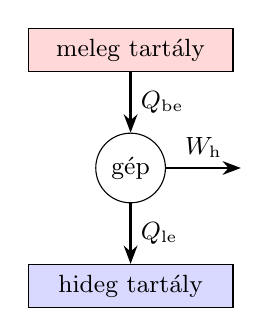
\begin{tikzpicture}[font=\small]
    \node[draw,fill=red!15,minimum width=2.6cm,minimum height=0.55cm] (M) at (0,1.5) {meleg tartály};
    \node[draw,circle,minimum size=0.75cm] (G) at (0,0) {gép};
    \node[draw,fill=blue!15,minimum width=2.6cm,minimum height=0.55cm] (H) at (0,-1.5) {hideg tartály};
    \draw[-{Stealth},thick] (M) -- node[right] {$Q_\text{be}$} (G);
    \draw[-{Stealth},thick] (G) -- node[right] {$Q_\text{le}$} (H);
    \draw[-{Stealth},thick] (G) -- node[above] {$W_\text{h}$} (1.4,0);
  \end{tikzpicture}\\[2pt]
  {\small (hőerőgép vázlata)}\\[8pt]
  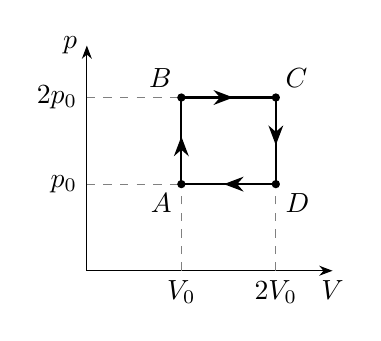
\begin{tikzpicture}[x=1.2cm,y=1.1cm]
    \draw[-{Stealth}] (0,0) -- (2.6,0) node[below] {$V$};
    \draw[-{Stealth}] (0,0) -- (0,2.6) node[left] {$p$};
    \draw[dashed,gray] (1,0) node[below,black] {$V_0$} -- (1,1);
    \draw[dashed,gray] (2,0) node[below,black] {$2V_0$} -- (2,1);
    \draw[dashed,gray] (0,1) node[left,black] {$p_0$} -- (1,1);
    \draw[dashed,gray] (0,2) node[left,black] {$2p_0$} -- (1,2);
    \draw[thick,midarrow] (1,1) -- (1,2);
    \draw[thick,midarrow] (1,2) -- (2,2);
    \draw[thick,midarrow] (2,2) -- (2,1);
    \draw[thick,midarrow] (2,1) -- (1,1);
    \foreach \p/\n/\pos in {{(1,1)}/A/below left, {(1,2)}/B/above left,
                            {(2,2)}/C/above right, {(2,1)}/D/below right}
      \fill \p circle (1.5pt) node[\pos] {$\n$};
  \end{tikzpicture}\\[2pt]
  {\small (2.~feladat: az előző órai körfolyamat)}
\end{minipage}

\newpage
\begin{enumerate}[start=5]
\item \textbf{Perpetuum mobile.}
  \textbf{a)} Mi az elsőfajú és mi a másodfajú perpetuum mobile? Melyik főtételt sértené
  az egyik, és melyiket a másik?
  \textbf{b)} Döntsd el az alábbi ötletekről, hogy elsőfajú vagy másodfajú perpetuum
  mobile-e, vagy működhet! Indokold!
  \begin{enumerate}
    \item Egy kerék küllőire csuklósan súlyokat erősítünk. Az egyik oldalon a súlyok
      kihajlanak, ezért a feltaláló szerint az az oldal mindig ,,nehezebb'', így a kerék
      örökké forog, és közben munkát is végez.
    \item Egy villanymotor egy generátort hajt, a generátor árama táplálja a motort, és a
      ,,felesleg'' még egy izzót is működtet.
    \item Egy hajó a tengervízből hőt von el, és ezt teljes egészében a hajócsavar
      meghajtására fordítja; a lehűlt vizet visszaengedi a tengerbe. Miért nem segít,
      hogy a tenger belső energiája óriási?
    \item Egy trópusi erőmű a $25\,^\circ$C-os felszíni és a mélyből felszivattyúzott
      $5\,^\circ$C-os víz hőmérséklet-különbségét hasznosítja. Mekkora lehet legfeljebb
      a hatásfoka?
  \end{enumerate}
  \textbf{c)} Hogyan függ össze a 4.\,c) feladat folyamata a másodfajú perpetuum
  mobile-val?

\item Összefüggő szöveggel, néhány mondatban fejtsd ki, hogyan működik egy hőerőgép, és
  miért van szükség hideg tartályra is! (Itt a szabatos szöveges kifejtés a lényeg, ezt
  pontozzák az érettségin.)
\end{enumerate}

\end{document}
